%MKB
%Mathematik 2
%�bungseinheit 3

%Einbinden der Aufgaben
\insertrep{MKB/UE_03/Uebungseinheit-3_Parallelprojektion_Axonometrie.pdf}{"Ubungseinheit 3}

%Praesenzaufgaben
%MKB
%Mathematik
%Übungseinheit 3
%Hausübungen
%Aufgabe P5


\setcounter{P-section}{5}
\renewcommand*\thesection{P\Nummerierung{\arabic{P-section}}}
\section{Analyse einiger Kavalierprojektionen}


%MKB
%Mathematik
%Übungseinheit 3
%Hausübungen
%Aufgabe P6

\setcounter{P-section}{6}
\renewcommand*\thesection{P\Nummerierung{\arabic{P-section}}}
\section{Fortsetzung der Analyse – Projektion auf verschiedene Ebenen}

%MKB
%Mathematik
%Übungseinheit 3
%Hausübungen
%Aufgabe P7 
\pagebreak
\setcounter{P-section}{7}
\renewcommand*\thesection{P\Nummerierung{\arabic{P-section}}}
\section{Kuboktaeder}

\begin{center}
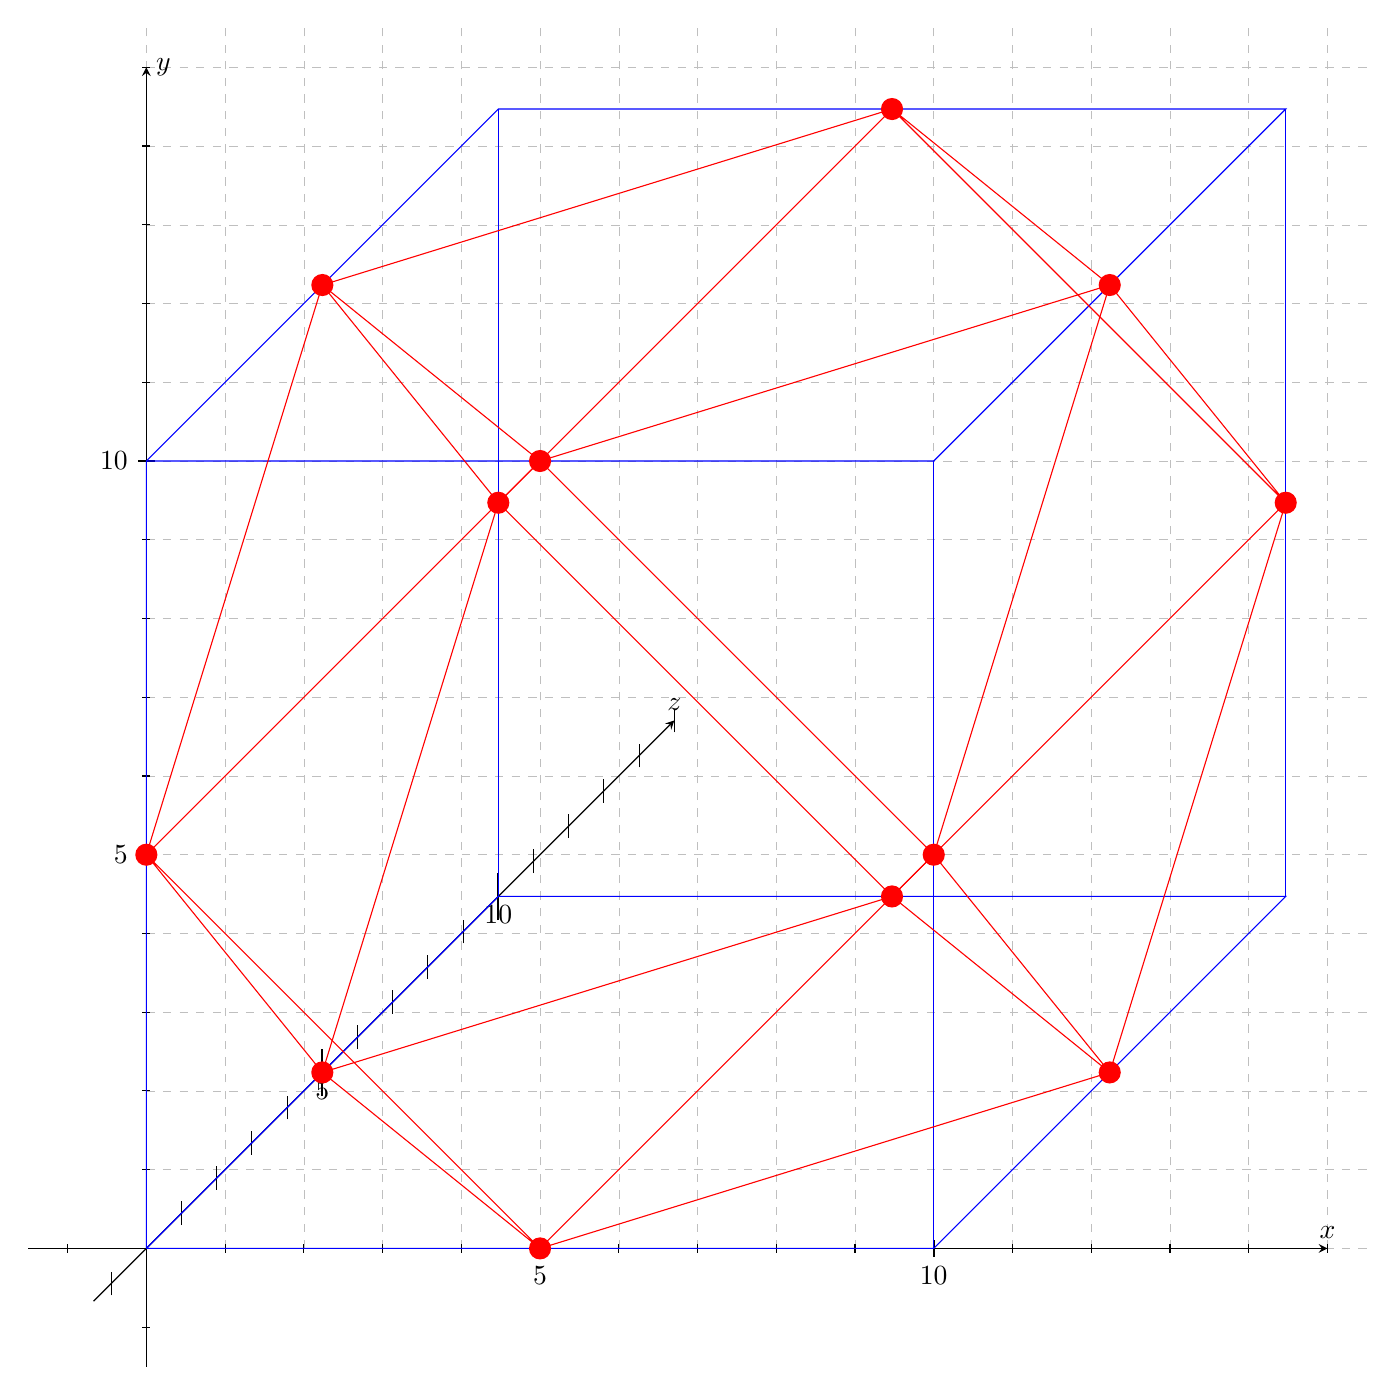
\begin{tikzpicture}[x=1cm,y=1cm,z=0.447cm,>=stealth]
\draw[step=1cm,lightgray,very thin,dashed] (0,15.5) grid (15.5,0);
% The axes
\draw[->] (xyz cs:x=-1.5) -- (xyz cs:x=15) node[above] {$x$};
\draw[->] (xyz cs:y=-1.5) -- (xyz cs:y=15) node[right] {$y$};
\draw[->] (xyz cs:z=-1.5) -- (xyz cs:z=15) node[above] {$z$};
% The thin ticks

\foreach \coo in {-1,0,...,15.5}
{
	\draw (\coo,-1.5pt) -- (\coo,1.5pt);
	\draw (-1.5pt,\coo) -- (1.5pt,\coo);
	\draw (xyz cs:y=-0.15pt,z=\coo) -- (xyz cs:y=0.15pt,z=\coo);
}

% The thick ticks
\foreach \coo in {5,10}
{
	\draw[thick] (\coo,-3pt) -- (\coo,3pt) node[below=6pt] {\coo};
	\draw[thick] (-3pt,\coo) -- (3pt,\coo) node[left=6pt] {\coo};
	\draw[thick] (xyz cs:y=-0.3pt,z=\coo) -- (xyz cs:y=0.3pt,z=\coo) node[below=8pt] {\coo};
}

% Dashed lines for the points P, Q
%\draw[dashed] 
%(xyz cs:z=0) -- +(0,10) -- (xyz cs:y=10) -- +(10,0) -- ++(xyz cs:x=10,z=10) -- +(-10,0) --  ++(xyz cs:x=0,z=0)--+(0,-10);% --cycle;

\draw[blue] (xyz cs:z=0) -- +(0,10)--(xyz cs:y=10)-- +(10,0)--(xyz cs:x=10,y=10,z=10)--+(-10,0)--(xyz cs:x=0,y=10,z=0) ;% --cycle;

\draw[blue] (xyz cs:z=0) -- +(10,0)-- (xyz cs:x=10,z=10)--+(-10,0)--(xyz cs:x=0,z=0);

\draw[blue] (xyz cs:x=10,y=0,z=0) -- (xyz cs:x=10,y=10,z=0);
\draw[blue] (xyz cs:x=10,y=0,z=10) -- (xyz cs:x=10,y=10,z=10);
\draw[blue] (xyz cs:x=0,y=0,z=10) -- (xyz cs:x=0,y=10,z=10);

%Above 
\draw[red] (xyz cs:x=0,y=5,z=0) -- (xyz cs:x=5,y=10,z=0)--(xyz cs:x=0,y=10,z=5)--(xyz cs:x=0,y=5,z=0);
\draw[red] (xyz cs:x=0,y=10,z=5) -- (xyz cs:x=0,y=5,z=10)--(xyz cs:x=5,y=10,z=10)--(xyz cs:x=0,y=10,z=5);
\draw[red] (xyz cs:x=5,y=10,z=10) -- (xyz cs:x=10,y=5,z=10)--(xyz cs:x=10,y=10,z=5)--(xyz cs:x=5,y=10,z=10);
\draw[red] (xyz cs:x=10,y=10,z=5) -- (xyz cs:x=10,y=5,z=0)--(xyz cs:x=5,y=10,z=0)--(xyz cs:x=10,y=10,z=5);

%Bottom
\draw[red] (xyz cs:x=0,y=5,z=0) -- (xyz cs:x=0,y=0,z=5)--(xyz cs:x=5,y=0,z=0)--(xyz cs:x=0,y=5,z=0);
\draw[red] (xyz cs:x=0,y=0,z=5) -- (xyz cs:x=0,y=5,z=10)--(xyz cs:x=5,y=0,z=10)--(xyz cs:x=0,y=0,z=5);
\draw[red] (xyz cs:x=5,y=0,z=10) -- (xyz cs:x=10,y=5,z=10)--(xyz cs:x=10,y=0,z=5)--(xyz cs:x=5,y=0,z=10);
\draw[red] (xyz cs:x=5,y=0,z=0) -- (xyz cs:x=10,y=5,z=0)--(xyz cs:x=10,y=0,z=5)--(xyz cs:x=5,y=0,z=0);

\fill[red] (xyz cs:x=0,y=5,z=0) circle (4pt);
\fill[red] (xyz cs:x=5,y=10,z=0) circle (4pt);
\fill[red] (xyz cs:x=0,y=10,z=5) circle (4pt);
\fill[red] (xyz cs:x=0,y=5,z=10) circle (4pt);
\fill[red] (xyz cs:x=5,y=10,z=10) circle (4pt);
\fill[red] (xyz cs:x=10,y=10,z=5) circle (4pt);
\fill[red] (xyz cs:x=10,y=5,z=10) circle (4pt);
\fill[red] (xyz cs:x=10,y=5,z=0) circle (4pt);
\fill[red] (xyz cs:x=10,y=0,z=5) circle (4pt);
\fill[red] (xyz cs:x=5,y=0,z=10) circle (4pt);
\fill[red] (xyz cs:x=0,y=0,z=5) circle (4pt);
\fill[red] (xyz cs:x=5,y=0,z=0) circle (4pt);

\end{tikzpicture}
\end{center}
\textbf{Kuboktaeder:} \\
\\
Ecken($e$): 12\\
\\
Kanten($k$): 24\\
\\
Fl"achen:($f$): 14\\
\\
Die eulersche Polyederformel lautet: e - k + f = 2. Wenn man die Werte f"ur die Ecken, Kanten und Fl"achen des Kuboktaeder einsetzt bekommt man: 12 - 24 + 14 = 2. Daraus erschlie"st sich, dass die eulersche Polyederformel erf"ullt ist.

%Hausuebungen
%MKB
%Mathematik 2
%Übungseinheit 3
%Hausübungen
%Aufgabe H3

\setcounter{H-section}{3}
\renewcommand*\thesection{H\Nummerierung{\arabic{H-section}}}
\section{Castellum}


\begin{tikzpicture}[x=1cm,y=1cm,z=0.5cm,>=stealth]

\draw[step=1cm,lightgray,very thin,dashed] (0,13.5) grid (13.5,0);

% The axes
\draw[->] (xyz cs:x=-1.5) -- (xyz cs:x=13.5) node[above] {$x$};
\draw[->] (xyz cs:y=-1.5) -- (xyz cs:y=13.5) node[right] {$y$};
\draw[->] (xyz cs:z=-1.5) -- (xyz cs:z=13.5) node[above] {$z$};
% The thin ticks

\foreach \coo in {-1,0,...,13}
{
	\draw (\coo,-1.5pt) -- (\coo,1.5pt);
	\draw (-1.5pt,\coo) -- (1.5pt,\coo);
	\draw (xyz cs:y=-0.15pt,z=\coo) -- (xyz cs:y=0.15pt,z=\coo);
}

% The thick ticks
\foreach \coo in {5,10}
{
	\draw[thick] (\coo,-3pt) -- (\coo,3pt) node[below=6pt] {\coo};
	\draw[thick] (-3pt,\coo) -- (3pt,\coo) node[left=6pt] {\coo};
	\draw[thick] (xyz cs:y=-0.3pt,z=\coo) -- (xyz cs:y=0.3pt,z=\coo) node[below=8pt] {\coo};
}

%Tower left front
\draw[blue] (xyz cs:z=0) -- +(0,5)--(xyz cs:y=5)-- +(2,0)--+(2,-5)--cycle;
\draw[blue] (xyz cs:x=0,y=5,z=0)--+(0,0,2)--+(2,0,2)--+(2,0,0);
\draw[blue] (xyz cs:x=2,y=5,z=2)--+(0,-2,0)--+(0,-2,-1)--+(0,-5,-1)--+(0,-5,-2);

\draw[blue] (xyz cs:x=0.5,y=5,z=0.5)--+(1,0,0)--+(1,0,1)--+(0,0,1)--cycle;

%Tower right front
\draw[blue] (xyz cs:x=6,y=0,z=0)--+(0,5,0)--+(2,5,0)--+(2,0,0)--cycle;
\draw[blue] (xyz cs:x=6,y=5,z=0)--+(0,0,2)--+(2,0,2)--+(2,0,0);
\draw[blue] (xyz cs:x=8,y=5,z=2)--+(0,-5,0)--+(0,-5,-2);

\draw[blue] (xyz cs:x=6.5,y=5,z=0.5)--+(1,0,0)--+(1,0,1)--+(0,0,1)--cycle;

%Tower left back
\draw[blue] (xyz cs:x=0,y=0,z=6)--+(0,5,0)--+(2,5,0)--+(2,1,0);
\draw[blue] (xyz cs:x=0,y=5,z=6)--+(0,0,2)--+(2,0,2)--+(2,0,0);
\draw[blue] (xyz cs:x=2,y=5,z=8)--+(0,-2.5,0);

\draw[blue] (xyz cs:x=0.5,y=5,z=6.5)--+(1,0,0)--+(1,0,1)--+(0,0,1)--cycle;

%Tower right back
\draw[blue] (xyz cs:x=8,y=0,z=6)--+(0,5,0)--+(-2,5,0)--+(-2,3,0)--+(-1,3,0)--+(-1,0,0)--cycle;
\draw[blue] (xyz cs:x=8,y=0,z=6)--+(0,0,2)--+(0,5,2)--+(0,5,0);
\draw[blue] (xyz cs:x=8,y=5,z=8)--+(-2,0,0)--+(-2,0,-2);

\draw[blue] (xyz cs:x=6.5,y=5,z=6.5)--+(1,0,0)--+(1,0,1)--+(0,0,1)--cycle;


%Wall back
\draw[blue] (xyz cs:x=2,y=3,z=6)--+(4,0,0);
\draw[blue] (xyz cs:x=2,y=3,z=6)--+(0,0,1);
\draw[blue] (xyz cs:x=2,y=3,z=7)--+(3.5,0,0);

%Wall left
\draw[blue] (xyz cs:x=2,y=3,z=6)--+(0,0,-4);
\draw[blue] (xyz cs:x=2,y=3,z=6)--+(-1,0,0);
\draw[blue] (xyz cs:x=1,y=3,z=6)--+(0,0,-2);

%Wall right
\draw[blue] (xyz cs:x=7,y=3,z=6)--+(0,0,-2);
\draw[blue] (xyz cs:x=7,y=0,z=6)--+(0,0,-2);

%Wall front
\draw[blue] (xyz cs:x=2,y=3,z=2)--+(3,0,0);
\draw[blue] (xyz cs:x=2,y=3,z=1)--+(3.5,0,0);
\draw[blue] (xyz cs:x=2,y=0,z=1)--+(3.5,0,0);

%\draw[blue] (xyz cs:z=0) -- +(10,0)-- (xyz cs:x=10,z=10)--+(-10,0)--(xyz cs:x=0,z=0);
%
%\draw[blue] (xyz cs:x=10,y=0,z=0) -- (xyz cs:x=10,y=10,z=0);
%\draw[blue] (xyz cs:x=10,y=0,z=10) -- (xyz cs:x=10,y=10,z=10);
%\draw[blue] (xyz cs:x=0,y=0,z=10) -- (xyz cs:x=0,y=10,z=10);



\node[align=center] at (3,-3) (ori) {(0,0,0)\\\text{origin}};
\draw[->,help lines,shorten >=3pt] (ori) .. controls (1,-2) and (1.2,-1.5) .. (0,0,0);
\end{tikzpicture}
%MKB
%Mathematik 2
%Übungseinheit 3
%Hausübungen
%Aufgabe H4

\setcounter{H-section}{4}
\renewcommand*\thesection{H\Nummerierung{\arabic{H-section}}}
\section{Dynamische veränderbare Darstellungen mit Geogebra}


aiohsogihaoihroighaeorhg
%%MKB
%Mathematik 2
%Übungseinheit 3
%Hausübungen
%Aufgabe H3

\setcounter{H-section}{3}
\renewcommand*\thesection{H\Nummerierung{\arabic{H-section}}}
\section{Castellum}


\begin{tikzpicture}[x=1cm,y=1cm,z=0.5cm,>=stealth]

\draw[step=1cm,lightgray,very thin,dashed] (0,13.5) grid (13.5,0);

% The axes
\draw[->] (xyz cs:x=-1.5) -- (xyz cs:x=13.5) node[above] {$x$};
\draw[->] (xyz cs:y=-1.5) -- (xyz cs:y=13.5) node[right] {$y$};
\draw[->] (xyz cs:z=-1.5) -- (xyz cs:z=13.5) node[above] {$z$};
% The thin ticks

\foreach \coo in {-1,0,...,13}
{
	\draw (\coo,-1.5pt) -- (\coo,1.5pt);
	\draw (-1.5pt,\coo) -- (1.5pt,\coo);
	\draw (xyz cs:y=-0.15pt,z=\coo) -- (xyz cs:y=0.15pt,z=\coo);
}

% The thick ticks
\foreach \coo in {5,10}
{
	\draw[thick] (\coo,-3pt) -- (\coo,3pt) node[below=6pt] {\coo};
	\draw[thick] (-3pt,\coo) -- (3pt,\coo) node[left=6pt] {\coo};
	\draw[thick] (xyz cs:y=-0.3pt,z=\coo) -- (xyz cs:y=0.3pt,z=\coo) node[below=8pt] {\coo};
}

%Tower left front
\draw[blue] (xyz cs:z=0) -- +(0,5)--(xyz cs:y=5)-- +(2,0)--+(2,-5)--cycle;
\draw[blue] (xyz cs:x=0,y=5,z=0)--+(0,0,2)--+(2,0,2)--+(2,0,0);
\draw[blue] (xyz cs:x=2,y=5,z=2)--+(0,-2,0)--+(0,-2,-1)--+(0,-5,-1)--+(0,-5,-2);

\draw[blue] (xyz cs:x=0.5,y=5,z=0.5)--+(1,0,0)--+(1,0,1)--+(0,0,1)--cycle;

%Tower right front
\draw[blue] (xyz cs:x=6,y=0,z=0)--+(0,5,0)--+(2,5,0)--+(2,0,0)--cycle;
\draw[blue] (xyz cs:x=6,y=5,z=0)--+(0,0,2)--+(2,0,2)--+(2,0,0);
\draw[blue] (xyz cs:x=8,y=5,z=2)--+(0,-5,0)--+(0,-5,-2);

\draw[blue] (xyz cs:x=6.5,y=5,z=0.5)--+(1,0,0)--+(1,0,1)--+(0,0,1)--cycle;

%Tower left back
\draw[blue] (xyz cs:x=0,y=0,z=6)--+(0,5,0)--+(2,5,0)--+(2,1,0);
\draw[blue] (xyz cs:x=0,y=5,z=6)--+(0,0,2)--+(2,0,2)--+(2,0,0);
\draw[blue] (xyz cs:x=2,y=5,z=8)--+(0,-2.5,0);

\draw[blue] (xyz cs:x=0.5,y=5,z=6.5)--+(1,0,0)--+(1,0,1)--+(0,0,1)--cycle;

%Tower right back
\draw[blue] (xyz cs:x=8,y=0,z=6)--+(0,5,0)--+(-2,5,0)--+(-2,3,0)--+(-1,3,0)--+(-1,0,0)--cycle;
\draw[blue] (xyz cs:x=8,y=0,z=6)--+(0,0,2)--+(0,5,2)--+(0,5,0);
\draw[blue] (xyz cs:x=8,y=5,z=8)--+(-2,0,0)--+(-2,0,-2);

\draw[blue] (xyz cs:x=6.5,y=5,z=6.5)--+(1,0,0)--+(1,0,1)--+(0,0,1)--cycle;


%Wall back
\draw[blue] (xyz cs:x=2,y=3,z=6)--+(4,0,0);
\draw[blue] (xyz cs:x=2,y=3,z=6)--+(0,0,1);
\draw[blue] (xyz cs:x=2,y=3,z=7)--+(3.5,0,0);

%Wall left
\draw[blue] (xyz cs:x=2,y=3,z=6)--+(0,0,-4);
\draw[blue] (xyz cs:x=2,y=3,z=6)--+(-1,0,0);
\draw[blue] (xyz cs:x=1,y=3,z=6)--+(0,0,-2);

%Wall right
\draw[blue] (xyz cs:x=7,y=3,z=6)--+(0,0,-2);
\draw[blue] (xyz cs:x=7,y=0,z=6)--+(0,0,-2);

%Wall front
\draw[blue] (xyz cs:x=2,y=3,z=2)--+(3,0,0);
\draw[blue] (xyz cs:x=2,y=3,z=1)--+(3.5,0,0);
\draw[blue] (xyz cs:x=2,y=0,z=1)--+(3.5,0,0);

%\draw[blue] (xyz cs:z=0) -- +(10,0)-- (xyz cs:x=10,z=10)--+(-10,0)--(xyz cs:x=0,z=0);
%
%\draw[blue] (xyz cs:x=10,y=0,z=0) -- (xyz cs:x=10,y=10,z=0);
%\draw[blue] (xyz cs:x=10,y=0,z=10) -- (xyz cs:x=10,y=10,z=10);
%\draw[blue] (xyz cs:x=0,y=0,z=10) -- (xyz cs:x=0,y=10,z=10);



\node[align=center] at (3,-3) (ori) {(0,0,0)\\\text{origin}};
\draw[->,help lines,shorten >=3pt] (ori) .. controls (1,-2) and (1.2,-1.5) .. (0,0,0);
\end{tikzpicture}

%Tutoriumsuebungen
%Mathematik 2
%Übungseinheit 3
%Hausübungen
%Aufgabe T1

\setcounter{T-section}{1}
\renewcommand*\thesection{T\Nummerierung{\arabic{T-section}}}
\section{Parallelprojektionen in die Aufrissebene}


a)\\
\begin{center}
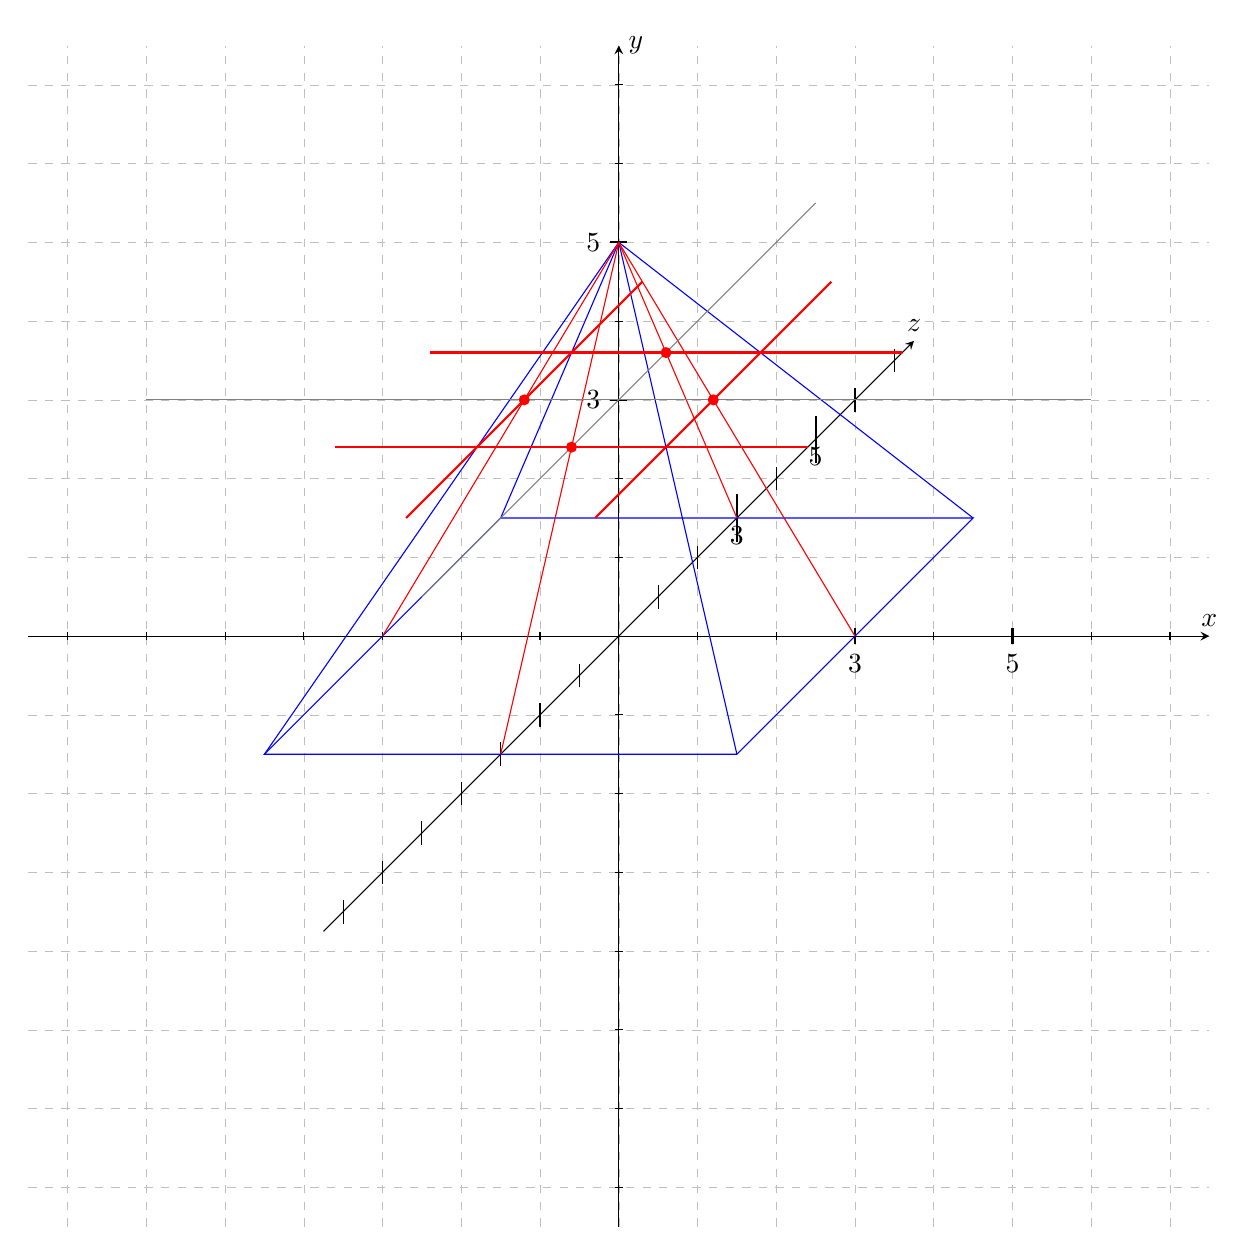
\begin{tikzpicture}[x=1cm,y=1cm,z=0.5cm,>=stealth]

\draw[step=1cm,lightgray,very thin,dashed] (-7.5,7.5) grid (7.5,-7.5);

% The axes
\draw[->] (xyz cs:x=-7.5) -- (xyz cs:x=7.5) node[above] {$x$};
\draw[->] (xyz cs:y=-7.5) -- (xyz cs:y=7.5) node[right] {$y$};
\draw[->] (xyz cs:z=-7.5) -- (xyz cs:z=7.5) node[above] {$z$};
% The thin ticks

\foreach \coo in {-7,...,7}
{
	\draw (\coo,-1.5pt) -- (\coo,1.5pt);
	\draw (-1.5pt,\coo) -- (1.5pt,\coo);
	\draw (xyz cs:y=-0.15pt,z=\coo) -- (xyz cs:y=0.15pt,z=\coo);
}

% The thick ticks
\foreach \coo in {3,5}
{
	\draw[thick] (\coo,-3pt) -- (\coo,3pt) node[below=6pt] {\coo};
	\draw[thick] (-3pt,\coo) -- (3pt,\coo) node[left=6pt] {\coo};
	\draw[thick] (xyz cs:y=-0.3pt,z=\coo) -- (xyz cs:y=0.3pt,z=\coo) node[below=8pt] {\coo};
}

\draw[blue] (xyz cs:x=-3,y=0,z=-3)--+(6,0,0)--+(6,0,6)--+(0,0,6)--cycle;
\draw[blue] (xyz cs:x=0,y=5,z=0)--+(-3,-5,-3);
\draw[blue] (xyz cs:x=0,y=5,z=0)--+(3,-5,3);
\draw[blue] (xyz cs:x=0,y=5,z=0)--+(3,-5,-3);
\draw[blue] (xyz cs:x=0,y=5,z=0)--+(-3,-5,3);


%Seitenhalbierende
\draw[red] (xyz cs:x=0,y=0,z=-3)coordinate(s_1)--(xyz cs:x=0,y=5,z=0)coordinate(s_11);
\draw[red] (xyz cs:x=3,y=0,z=0)coordinate(s_2)--+(-3,5,0)coordinate(s_22);
\draw[red] (xyz cs:x=0,y=0,z=3)coordinate(s_3)--+(0,5,-3)coordinate(s_33);
\draw[red] (xyz cs:x=-3,y=0,z=0)coordinate(s_4)--+(3,5,0)coordinate(s_44);

%verschieben des Koordinatensystems in Punkt 3
\draw[gray] (xyz cs:x=0,y=3,z=-5)coordinate(k_1)--(xyz cs:x=0,y=3,z=5)coordinate(k_11);
\draw[gray] (xyz cs:x=-6,y=3,z=0)coordinate(k_2)--(xyz cs:x=6,y=3,z=0)coordinate(k_22);

%Schnittpunkte Seitenhalbierende und Koordinatenachsen
\coordinate (c) at (intersection of s_1--s_11 and k_1--k_11);
\fill[red](c) circle(2pt);
\coordinate (d) at (intersection of s_2--s_22 and k_2--k_22);
\fill[red](d) circle(2pt);
\coordinate (e) at (intersection of s_3--s_33 and k_1--k_11);
\fill[red](e) circle(2pt);
\coordinate (f) at (intersection of s_4--s_44 and k_2--k_22);
\fill[red](f) circle(2pt);

\draw[red, thick] (c)--+(3,0,0)--+(-3,0,0);
\draw[red, thick] (e)--+(3,0,0)--+(-3,0,0);
\draw[red, thick] (d)--+(0,0,3)--+(0,0,-3);
\draw[red, thick] (f)--+(0,0,3)--+(0,0,-3);

\end{tikzpicture}
\end{center}
\usetikzlibrary{calc}
\pagebreak
b)
\begin{center}
\begin{tikzpicture}[x=1.5cm,y=1.5cm,z=0.75cm,>=stealth]

\draw[step=1.5cm,lightgray,very thin,dashed] (-5.5,5.5) grid (5.5,-5.5);

% The axes
\draw[->] (xyz cs:x=-5.5) -- (xyz cs:x=5.5) node[above] {$x$};
\draw[->] (xyz cs:y=-5.5) -- (xyz cs:y=5.5) node[right] {$z$};
\draw[->] (xyz cs:z=-5.5) -- (xyz cs:z=5.5) node[above] {$y$};
% The thin ticks

\foreach \coo in {-5,...,5}
{
	\draw (\coo,-5.5pt) -- (\coo,1.5pt);
	\draw (-5.5pt,\coo) -- (1.5pt,\coo);
	\draw (xyz cs:y=-0.15pt,z=\coo) -- (xyz cs:y=0.15pt,z=\coo);
}

% The thick ticks
\foreach \coo in {5}
{
	\draw[thick] (\coo,-3pt) -- (\coo,3pt) node[below=6pt] {\coo};
	\draw[thick] (-3pt,\coo) -- (3pt,\coo) node[left=6pt] {\coo};
	\draw[thick] (xyz cs:y=-0.3pt,z=\coo) -- (xyz cs:y=0.3pt,z=\coo) node[below=8pt] {\coo};
}

\draw[blue](xyz cs: x=0,y=-3,z=0)--+(3,0,0)--+(3,6,0)--+(-3,6,0)--+(-3,0,0)--cycle;
\draw[red] (0,0) circle (4.5cm);

\fill[red](xyz cs: x=3,y=0,z=0) circle(3pt);
\fill[red](xyz cs: x=-3,y=0,z=0) circle(3pt);

\fill[red](xyz cs: x=0,y=3,z=0) circle(3pt);
\fill[red](xyz cs: x=0,y=-3,z=0) circle(3pt);


\end{tikzpicture}
\end{center}
\pagebreak
c)
\begin{center}
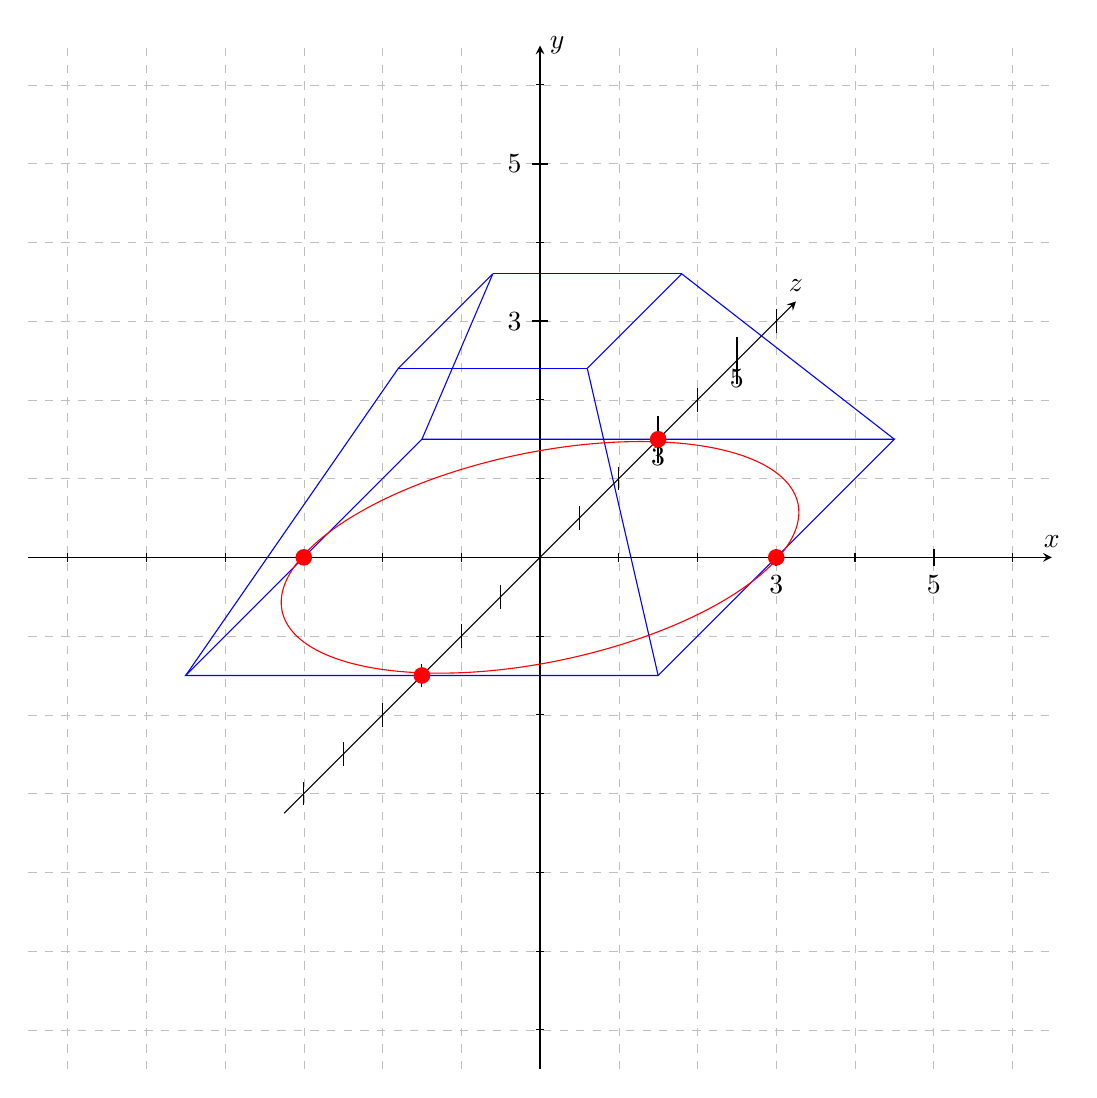
\begin{tikzpicture}[x=1cm,y=1cm,z=0.5cm,>=stealth]

\draw[step=1cm,lightgray,very thin,dashed] (-6.5,6.5) grid (6.5,-6.5);

% The axes
\draw[->] (xyz cs:x=-6.5) -- (xyz cs:x=6.5) node[above] {$x$};
\draw[->] (xyz cs:y=-6.5) -- (xyz cs:y=6.5) node[right] {$y$};
\draw[->] (xyz cs:z=-6.5) -- (xyz cs:z=6.5) node[above] {$z$};
% The thin ticks

\foreach \coo in {-6,...,6}
{
	\draw (\coo,-1.5pt) -- (\coo,1.5pt);
	\draw (-1.5pt,\coo) -- (1.5pt,\coo);
	\draw (xyz cs:y=-0.15pt,z=\coo) -- (xyz cs:y=0.15pt,z=\coo);
}

% The thick ticks
\foreach \coo in {3,5}
{
	\draw[thick] (\coo,-3pt) -- (\coo,3pt) node[below=6pt] {\coo};
	\draw[thick] (-3pt,\coo) -- (3pt,\coo) node[left=6pt] {\coo};
	\draw[thick] (xyz cs:y=-0.3pt,z=\coo) -- (xyz cs:y=0.3pt,z=\coo) node[below=8pt] {\coo};
}

\draw[blue] (xyz cs:x=-3,y=0,z=-3)--+(6,0,0)--+(6,0,6)--+(0,0,6)--cycle;

\draw[blue](xyz cs: x=-3,y=0,z=-3)--(xyz cs: x=-1.2,y=3,z=-1.2);
\draw[blue](xyz cs: x=3,y=0,z=-3)--(xyz cs: x=1.2,y=3,z=-1.2);
\draw[blue](xyz cs: x=3,y=0,z=3)--(xyz cs: x=1.2,y=3,z=1.2);
\draw[blue](xyz cs: x=-3,y=0,z=3)--(xyz cs: x=-1.2,y=3,z=1.2);

\draw[blue](xyz cs: x=-1.2,y=3,z=1.2)--(xyz cs: x=1.2,y=3,z=1.2);
\draw[blue](xyz cs: x=-1.2,y=3,z=-1.2)--(xyz cs: x=1.2,y=3,z=-1.2);
\draw[blue](xyz cs: x=-1.2,y=3,z=-1.2)--(xyz cs: x=-1.2,y=3,z=1.2);
\draw[blue](xyz cs: x=1.2,y=3,z=-1.2)--(xyz cs: x=1.2,y=3,z=1.2);

%\draw[red] (0,0,0) ellipse (3cm and 0cm and 1.5cm);
\begin{scope}[shift={(-1.2,-1.5))},x={(1.2,1.5)},y={($(-1.5,-1.5)!1!90:(1.5,1.5)$)}]
\draw[red] (1,0) ellipse (0.98 and 0.33);
\end{scope}

\fill[red](xyz cs: x=3,y=0,z=0) circle(3pt);
\fill[red](xyz cs: x=-3,y=0,z=0) circle(3pt);
\fill[red](xyz cs: x=0,y=0,z=-3) circle(3pt);
\fill[red](xyz cs: x=0,y=0,z=3) circle(3pt);


\end{tikzpicture}
\end{center}

\pagebreak
d)\\

\begin{center}
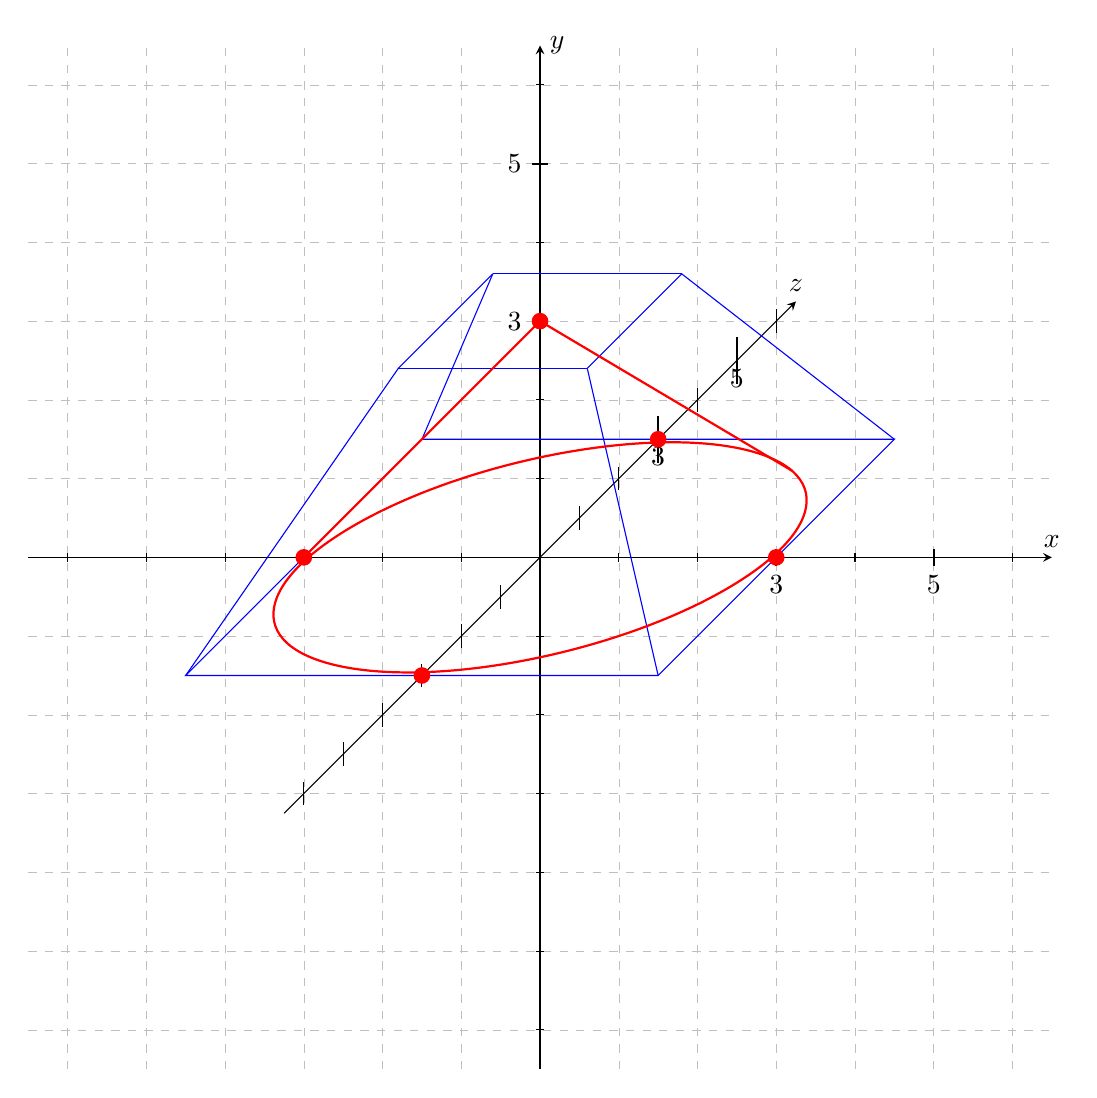
\begin{tikzpicture}[x=1cm,y=1cm,z=0.5cm,>=stealth]

\draw[step=1cm,lightgray,very thin,dashed] (-6.5,6.5) grid (6.5,-6.5);

% The axes
\draw[->] (xyz cs:x=-6.5) -- (xyz cs:x=6.5) node[above] {$x$};
\draw[->] (xyz cs:y=-6.5) -- (xyz cs:y=6.5) node[right] {$y$};
\draw[->] (xyz cs:z=-6.5) -- (xyz cs:z=6.5) node[above] {$z$};
% The thin ticks

\foreach \coo in {-6,...,6}
{
	\draw (\coo,-1.5pt) -- (\coo,1.5pt);
	\draw (-1.5pt,\coo) -- (1.5pt,\coo);
	\draw (xyz cs:y=-0.15pt,z=\coo) -- (xyz cs:y=0.15pt,z=\coo);
}

% The thick ticks
\foreach \coo in {3,5}
{
	\draw[thick] (\coo,-3pt) -- (\coo,3pt) node[below=6pt] {\coo};
	\draw[thick] (-3pt,\coo) -- (3pt,\coo) node[left=6pt] {\coo};
	\draw[thick] (xyz cs:y=-0.3pt,z=\coo) -- (xyz cs:y=0.3pt,z=\coo) node[below=8pt] {\coo};
}

\draw[blue] (xyz cs:x=-3,y=0,z=-3)--+(6,0,0)--+(6,0,6)--+(0,0,6)--cycle;

\draw[blue](xyz cs: x=-3,y=0,z=-3)--(xyz cs: x=-1.2,y=3,z=-1.2);
\draw[blue](xyz cs: x=3,y=0,z=-3)--(xyz cs: x=1.2,y=3,z=-1.2);
\draw[blue](xyz cs: x=3,y=0,z=3)--(xyz cs: x=1.2,y=3,z=1.2);
\draw[blue](xyz cs: x=-3,y=0,z=3)--(xyz cs: x=-1.2,y=3,z=1.2);

\draw[blue](xyz cs: x=-1.2,y=3,z=1.2)--(xyz cs: x=1.2,y=3,z=1.2);
\draw[blue](xyz cs: x=-1.2,y=3,z=-1.2)--(xyz cs: x=1.2,y=3,z=-1.2);
\draw[blue](xyz cs: x=-1.2,y=3,z=-1.2)--(xyz cs: x=-1.2,y=3,z=1.2);
\draw[blue](xyz cs: x=1.2,y=3,z=-1.2)--(xyz cs: x=1.2,y=3,z=1.2);


\begin{scope}[shift={(0,0))},x={(0.85,0.46)},y={($(-0.5,-0.3)!1!90:(0.5,0.3)$)}]
%\begin{scope}[shift={(-1.2,-1.5))},x={(1.2,1.5)},y={($(-1.5,-1.5)!1!90:(1.5,1.5)$)}]
%\draw[red,thick] (1,0) ellipse (0.98 and 0.33);
\draw[red,thick] (0,0) ellipse (3 and 1.5);
\end{scope}

%\draw[red,thick] (0,0) ellipse (3 and 1.5);

\fill[red](xyz cs: x=3,y=0,z=0) circle(3pt);
\fill[red](xyz cs: x=-3,y=0,z=0) circle(3pt);
\fill[red](xyz cs: x=0,y=0,z=-3) circle(3pt);
\fill[red](xyz cs: x=0,y=0,z=3) circle(3pt);

%Kegelstumpf
\fill[red](xyz cs: x=0,y=3,z=0) circle(3pt);
\draw[red,thick](xyz cs: x=0,y=3,z=0)--(xyz cs: x=-3,y=0,z=0);
\draw[red,thick](xyz cs: x=0,y=3,z=0)--(xyz cs: x=3.2,y=1.1,z=0);

\end{tikzpicture}
\end{center}



%Mathematik 2
%Übungseinheit 3
%Hausübungen
%Aufgabe T1

\setcounter{T-section}{2}
\renewcommand*\thesection{T\Nummerierung{\arabic{T-section}}}
\section{Parallelprojektionen in die Aufrissebene}

a)

Bild 1: \ensuremath{\theta =} 0$^{\circ}$ \; \ensuremath{\phi = 0}$^{\circ}$ \\
Bild 2:\ensuremath{\theta =} 0$^{\circ}$ \; \ensuremath{\phi = 90}$^{\circ}$ \\
Bild 3: \ensuremath{\theta =} 45$^{\circ}$ \; \ensuremath{\phi = 90}$^{\circ}$\\
%Mathematik 2
%Übungseinheit 3
%Hausübungen
%Aufgabe T1

\setcounter{T-section}{3}
\renewcommand*\thesection{T\Nummerierung{\arabic{T-section}}}
\section{Parallelprojektionen in die Aufrissebene}

\begin{center}
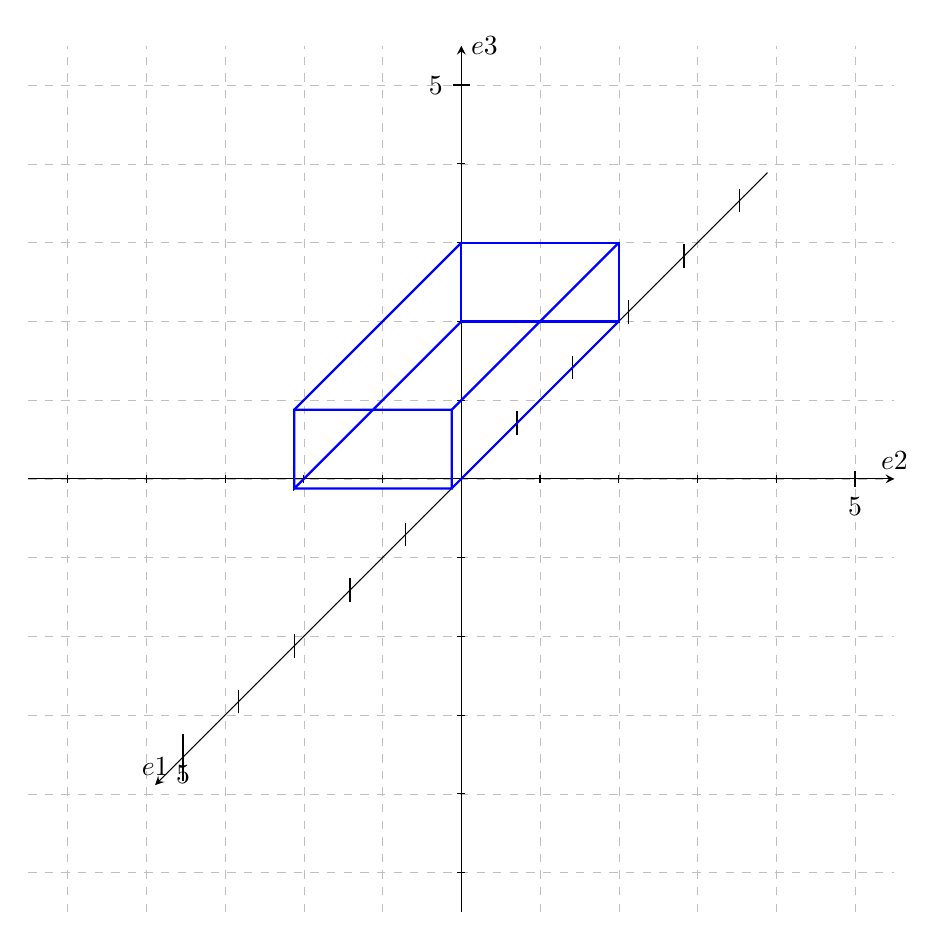
\begin{tikzpicture}[x=1cm,y=1cm,z=0.707cm,>=stealth]

\draw[step=1cm,lightgray,very thin,dashed] (-5.5,5.5) grid (5.5,-5.5);

% The axes
\draw[->] (xyz cs:x=-5.5) -- (xyz cs:x=5.5) node[above] {$e2$};
\draw[->] (xyz cs:y=-5.5) -- (xyz cs:y=5.5) node[right] {$e3$};
\draw[->] (xyz cs:z=5.5) -- (xyz cs:z=-5.5) node[above] {$e1$};
% The thin ticks

\foreach \coo in {-5,...,5}
{
	\draw (\coo,-1.5pt) -- (\coo,1.5pt);
	\draw (-1.5pt,\coo) -- (1.5pt,\coo);
	\draw (xyz cs:y=-0.15pt,z=\coo) -- (xyz cs:y=0.15pt,z=\coo);
}

% The thick ticks
\foreach \coo in {5}
{
	\draw[thick] (\coo,-3pt) -- (\coo,3pt) node[below=6pt] {\coo};
	\draw[thick] (-3pt,\coo) -- (3pt,\coo) node[left=6pt] {\coo};
	\draw[thick] (xyz cs:y=-0.3pt,z=-\coo) -- (xyz cs:y=0.3pt,z=-\coo) node[below=8pt] {\coo};
}

\draw[blue,thick] (xyz cs:x=0,y=2,z=0)--+(2,0,0)--+(2,1,0)--+(0,1,0)--cycle;
\draw[blue,thick] (xyz cs:x=0,y=2,z=0)--+(0,0,-3)--+(0,1,-3)--+(2,1,-3)--+(2,0,-3)--+(0,0,-3);
\draw[blue,thick] (xyz cs:x=2,y=2,z=0)--+(0,0,-3);
\draw[blue,thick] (xyz cs:x=0,y=3,z=0)--+(0,0,-3);
\draw[blue,thick] (xyz cs:x=2,y=3,z=0)--+(0,0,-3);

\end{tikzpicture}
\end{center}

\begin{center}
\begin{tikzpicture}[domain=0:2]
\draw[step=2cm,lightgray,very thin,dashed] (-7.5,7.5) grid (7.5,0);

\draw[->] (0,0) -- (7.5,0)
node[below right] {$x$};
\draw[->] (0,0) -- (0,7.5)
node[left] {$y$}; 
\draw[->] (0,0)--(-7.5,0)
node[left] {$z$};

\draw[blue,thick](0,4)--(4,4)--+(0,-2)--+(-4,-2)--cycle;
\draw[blue,thick](0,4)--(-6,4)--(-6,2)--(0,2);
\draw[blue,thick](-6,4)--(-6,2)--(-2,2)--(-2,4);


\end{tikzpicture}
\end{center}

%Mathematik 2
%Übungseinheit 3
%Hausübungen
%Aufgabe T1

\setcounter{T-section}{4}
\renewcommand*\thesection{T\Nummerierung{\arabic{T-section}}}
\section{Parallelprojektionen in die Aufrissebene}

\begin{center}
\begin{tikzpicture}[x=1cm,y=1cm,z=0.5cm,>=stealth]

\draw[step=1cm,lightgray,very thin,dashed] (-5.5,5.5) grid (5.5,-5.5);

% The axes
\draw[->] (xyz cs:x=-5.5) -- (xyz cs:x=5.5) node[above] {$e2$};
\draw[->] (xyz cs:y=-5.5) -- (xyz cs:y=5.5) node[right] {$e3$};
\draw[->] (xyz cs:z=5.5) -- (xyz cs:z=-5.5) node[above] {$e1$};
% The thin ticks

\foreach \coo in {-5,...,5}
{
	\draw (\coo,-1.5pt) -- (\coo,1.5pt);
	\draw (-1.5pt,\coo) -- (1.5pt,\coo);
	\draw (xyz cs:y=-0.15pt,z=\coo) -- (xyz cs:y=0.15pt,z=\coo);
}

% The thick ticks
\foreach \coo in {5}
{
	\draw[thick] (\coo,-3pt) -- (\coo,3pt) node[below=6pt] {\coo};
	\draw[thick] (-3pt,\coo) -- (3pt,\coo) node[left=6pt] {\coo};
	\draw[thick] (xyz cs:y=-0.3pt,z=-\coo) -- (xyz cs:y=0.3pt,z=-\coo) node[below=8pt] {\coo};
}

\fill[blue] (xyz cs:x=5,y=0,z=-2) circle (4pt) node[above] {$P'$};
\fill[blue] (xyz cs:x=5,y=4,z=-2) circle (4pt) node[above] {$P$};

\draw[dashed,blue,thick](xyz cs:x=5,y=0,z=-2)--(xyz cs:x=5,y=4,z=-2);

\draw[red](xyz cs:x=0,y=0,z=-2)--+(5,0,0)--+(5,0,2);

\end{tikzpicture}
\end{center}

P = (5,4,2);\\

\begin{center}
\begin{tikzpicture}[x=1cm,y=1cm,z=0.5cm,>=stealth]

\draw[step=1cm,lightgray,very thin,dashed] (-5.5,5.5) grid (5.5,-5.5);

% The axes
\draw[->] (xyz cs:x=-5.5) -- (xyz cs:x=5.5) node[above] {$e2$};
\draw[->] (xyz cs:y=-5.5) -- (xyz cs:y=5.5) node[right] {$e3$};
\draw[->] (xyz cs:z=5.5) -- (xyz cs:z=-5.5) node[above] {$e1$};
% The thin ticks

\foreach \coo in {-5,...,5}
{
	\draw (\coo,-1.5pt) -- (\coo,1.5pt);
	\draw (-1.5pt,\coo) -- (1.5pt,\coo);
	\draw (xyz cs:y=-0.15pt,z=\coo) -- (xyz cs:y=0.15pt,z=\coo);
}

% The thick ticks
\foreach \coo in {5}
{
	\draw[thick] (\coo,-3pt) -- (\coo,3pt) node[below=6pt] {\coo};
	\draw[thick] (-3pt,\coo) -- (3pt,\coo) node[left=6pt] {\coo};
	\draw[thick] (xyz cs:y=-0.3pt,z=-\coo) -- (xyz cs:y=0.3pt,z=-\coo) node[below=8pt] {\coo};
}

\fill[blue] (xyz cs:x=3,y=0,z=2) circle (4pt) node[below] {$P'$};
\fill[blue] (xyz cs:x=3,y=3,z=2) circle (4pt) node[above] {$P$};

\draw[dashed,blue,thick](xyz cs:x=3,y=0,z=2)--(xyz cs:x=3,y=3,z=2);

\draw[red](xyz cs:x=0,y=0,z=2)--+(3,0,0)--+(3,0,-2);

\end{tikzpicture}
\end{center}

P=(3,3,-2)